\documentclass[]{report}

\usepackage{amsmath,amsfonts}
\usepackage{graphicx}
\usepackage{url}
\usepackage[hidelinks]{hyperref}

% Title Page
\title{{\huge  TITLE} \\
{\small Automatic Control\\
Electronic Engineering for Intelligent Vehicles\\
University of Bologna\\
A.A. 202X-202X}}
\author{Student A and Student B and ...}


\begin{document}
\maketitle

\begin{abstract}
	Here briefly detail  the aims of the project.
\end{abstract}

\chapter{Introduction}
\section{Motivations}
Explain why the selected application is important. Describe the application with informal words.

\section{Contributions}
Describe what this project deals with. What has been done to solve the problem presented in the motivations.

\section{State of art and literature comparison}
List the closest works that deal with the same problem and compare the achievement obtained and the strategies exploited in this paper. For the search of the literature use \url{https://ieeexplore.ieee.org/Xplore/home.jsp} and \url{https://www.sciencedirect.com/}.

\section{Organisation of the manuscript}
Describe what the reader finds in each of the Sections of this manuscript.

\section{List of the symbols}
Here list all the symbols used in the manuscript and add a description to each of them (Use the International System of Units \url{https://en.wikipedia.org/wiki/International_System_of_Units}).

\chapter{MAIN BODY}
Change the title with the name of the selected application

\section{Model and Problem Formulation}
To define the control problem for the half-car active suspension system, we formalize the system as a nonlinear state-space model, which incorporates dynamics, sensor measurements, control inputs, and reference goals.

The system model is given by:
\begin{align}
	\dot{x} &= f(x, u, w) \\
	y &= h(x, u, w) \\
	e &= h_e(x, u, w)
\end{align}

Where:
\begin{itemize}
	\item $x \in \mathbb{R}^n$ is the \textbf{state vector},
	\item $u \in \mathbb{R}^p$ is the \textbf{control input vector},
	\item $y \in \mathbb{R}^q$ is the \textbf{measured output vector},
	\item $e \in \mathbb{R}^{l_m}$ is the \textbf{control error (goal)},
	\item $d \in \mathbb{R}^{l_d}$ is the \textbf{disturbance vector},
	\item $r \in \mathbb{R}^{l_r}$ is the \textbf{reference signal},
	\item $\nu \in \mathbb{R}^q$ is the \textbf{sensor noise},
	\item $w = \text{col}(d, \nu, r)$ is the \textbf{exogenous input}.
\end{itemize}
\begin{equation}
	\label{eq:FormulaA}
	\begin{aligned}
		\dot{x} &= f(x,u) && x(t_0) = x_0
\\
y &= h(x,u)
\end{aligned}
\end{equation}
\subsection*{Assumptions}

The control design relies on the following assumptions:

\begin{enumerate}
	\item The exogenous input $w$ is not directly measurable.
	\item Disturbances $d$ are bounded.
	\item Reference signal $r$ and its first derivatives are known.
	\item Bounded disturbances imply bounded internal states and outputs.
	\item The system has at least as many control inputs as control goals, i.e., $p \geq l_m$.
	\item The control error $e$ can be reconstructed from the output $y$: $\exists E$ such that $e = E(y)$.
\end{enumerate}

\section{Model Analysis}
\subsection{Dynamic Model}

The half-car model captures the vertical and roll dynamics of a vehicle subject to suspension forces and road disturbances. The state variables are:

\begin{align}
	x = \begin{bmatrix}
		x_1 \\ x_2 \\ x_3 \\ x_4 \\ x_5 \\ x_6
	\end{bmatrix} =
	\begin{bmatrix}
		z - z_g \\
		\dot{z} - \dot{z}_g \\
		\phi \\
		\dot{\phi} \\
		\phi_g \\
		\omega_g
	\end{bmatrix}
\end{align}

Control inputs are defined as:

\begin{align}
	u = \begin{bmatrix}
		u_1 \\
		u_2
	\end{bmatrix} =
	\begin{bmatrix}
		f_{al} + f_{ar} \\
		f_{al} d_l - f_{ar} d_r
	\end{bmatrix}
\end{align}

The system dynamics are expressed as:

\begin{align}
	\dot{x} = \begin{bmatrix}
		x_2 \\
		f_2 - \ddot{z}_g \\
		x_4 \\
		f_4 \\
		x_6 \\
		\alpha_g
	\end{bmatrix}
\end{align}

Where:
\begin{align}
	f_2 &= -g + \frac{1}{m}(f_{sl} + f_{sr}) + \frac{u_1}{m} \\
	f_4 &= \frac{1}{J}(f_{sl} d_l - f_{sr} d_r + u_2 + f_{wl} l + f_{wr} r)
\end{align}

The suspension deflections and velocities are:

\begin{align}
	s_1 &= x_1 + d_l(\sin x_3 - \sin x_5), \quad s_3 = x_1 - d_r(\sin x_3 - \sin x_5) \\
	s_2 &= x_2 + d_l(x_4 \cos x_3 - x_6 \cos x_5), \quad s_4 = x_2 - d_r(x_4 \cos x_3 - x_6 \cos x_5)
\end{align}

Suspension forces are modeled as spring-damper systems:

\begin{align}
	f_s(p, v) = -k p - \beta v
\end{align}

\subsection{Sensor Model}

The measurement vector is given by:

\begin{align}
	y = \begin{bmatrix}
		y_y \\
		y_z \\
		y_g \\
		y_l \\
		y_r
	\end{bmatrix} =
	\begin{bmatrix}
		\sin x_3(f_2 + g) + \cos x_3 \frac{f_{wr} + f_{wl}}{m} \\
		\cos x_3(f_2 + g) - \sin x_3 \frac{f_{wr} + f_{wl}}{m} \\
		x_4 \\
		s_1 \\
		s_3
	\end{bmatrix} + \nu
\end{align}

\subsection{Control Objectives}

We define the apparent roll angle $\phi_a$ using accelerometer data:

\begin{align}
	\phi_a = \sin^{-1} \left( \frac{y_y}{\sqrt{y_y^2 + y_z^2}} \right)
\end{align}

The control error vector is defined as:

\begin{align}
	e = \begin{bmatrix}
		\frac{y_l d_r + y_r d_l}{d_r + d_l} - r_z \\
		\phi_a - r_\phi
	\end{bmatrix}
\end{align}

This error describes deviations from the desired vertical height and perceived roll. The control task is to design $u$ to drive $e \rightarrow 0$ in the presence of disturbances and noise.

\section{Proposed Solution}
Here describe the proposed solution: Control system architecture (draw a block scheme!), mathematical description of the solution, listings of the MATLAB code implemented to obtain the solution

To include a picture use the environment \textit{figure}. 
\begin{figure}[h!]
	\centering
	%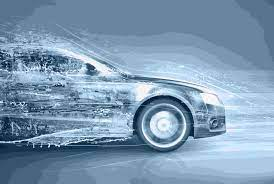
\includegraphics[width=0.7\columnwidth]{Figure}
	\caption{Add the caption to each figure! The caption should completely describe the figure so that the reader should be able to understand it without the need of reading the main text.}
	\label{fig:FigureA}
\end{figure}
Use the environment \textit{ref} to add a hyperlink to the figure. As example Figure \ref{fig:FigureA}.

\chapter{Application}

\section{Simulator description}
Copy and past the Simulink block scheme and describe what each block does. Describe the set-up MATLAB file, where and how to change the parameters of the simulations. Remember to include also the sensor noises and realistic external disturbances.

\section{Simulation results}
Describe the simulation scenario: initial conditions, purpose of the simulation. Describe the results: are the results coherent with the expectation? If not why? Investigate the tuning: how the performance are affected by the selection of the parameters at disposal of the designer?

\chapter{Conclusions and further investigation}
Recap the main results obtained in the project and highlight eventual further investigation directions alogn which the performance could be improved. 

\newpage
\chapter*{Bibliography}
List the papers/books cited.

\newpage
\appendix
\chapter*{Appendix}
Use appendices to add technical parts which are instrumental for the completeness of the manuscript but are too heavy to be included inside the main text. Basically, appendices are exploited to let the main text cleaner and smoother. As example, the complete MATLAB listings can be reported in appendix.\\

HO

\end{document}          
